% ===========================================================================
\section{Analysis}
\label{sec:analysis}
% ===========================================================================

The results above are three cells of a larger grid. This section walks the grid along the axes a reader would want to vary: how much midtraining and how much \ac{eft}; what is in the midtraining corpus and what is in the \ac{eft} mixture; whether the conflict touches one clause or all of them; whether the post-training is \ac{sft} or \ac{rl}; and whether the same pattern holds in a second setting.

\subsection{Scaling midtraining dose and \ac{eft} dose}
\label{sec:scaling}

\begin{figure}[t]
\centering

\includegraphics[width=\linewidth]{Figs/dose_response.pdf}
\caption{Charter-crew rate on held-in-clause, held-out-template conflict episodes against presented Charter tokens, for Gemma~3 12B (left) and 27B (right). One line per \ac{eft} dose (none, one epoch, two epochs); control dashed. \todo{Add the GLM-4.5-Air 1B-token run (lands 2026-09-10) as a third panel or an annotated point; it has no matched control.}}
\label{fig:dose_response}
\end{figure}

\paragraph{More midtraining helps, and the effect has not saturated.} Holding \ac{eft} fixed at two epochs of agreement-only data, the Charter-midtrained Gemma~3 27B model's Charter-crew rate rises from 48\% at 5M presented tokens to 62\% at 50M and 75\% at 190M, while the control stays between 26\% and 43\%. Gemma~3 12B shows the same monotone rise from 18\% at 1M to 65\% at 50M. Before \ac{eft}, every dose sits within a few points of 40\%, so the dose is expressed only once \ac{eft} has taught the task.

\paragraph{\ac{eft} dose barely matters within the range we ran.} One epoch and two epochs of agreement-only \ac{eft} give rates within the seed spread of each other at every midtraining dose. We also ran a tenfold \ac{eft} scale-up on GLM-4.5-Air (81{,}920 freshly generated agreement episodes, two epochs). The midtraining effect survives it: 81\% Charter against 23\% for the control at the end of training, and 91\% against 28\% at the one-epoch checkpoint. The tenfold scale-up does not, however, restore the held-out clauses (22\% at the end of training). \todo{Cells for 0.2\% and 10\% conflict at 81{,}920 rows are still landing; the 2\% Charter-labelled cell on the coin parent shows 22\% malformed answers and is probably over-trained (no replay mixture).}

\subsection{What is in the data}
\label{sec:data}

\begin{figure}[t]
\centering

\includegraphics[width=\linewidth]{Figs/no_worked_examples.pdf}
\caption{\textbf{Worked examples in the midtraining corpus carry most of the effect.} Charter-crew rate after agreement-only \ac{eft} (left) and after 2\% coin-labelled \ac{eft} (right) for Gemma~3 12B at 50M presented tokens, with the standard corpus and with the corpus restricted to documents that discuss the rule without an adjudicated example run. Control dashed. Under 2\% conflict both corpora fall to single digits.}
\label{fig:no_worked_examples}
\end{figure}

\paragraph{Half of the Charter corpus is worked examples, and they carry most of the effect.} Each clause appears in the corpus in two variants, one that walks a concrete adjudicated case and one that describes the practice without one. Restricting the corpus to the second variant at the same 50M dose cuts the Charter-midtrained model's rate after agreement-only \ac{eft} from 65\% to 37\%; the coin arm is unchanged (81\% and 79\% coin). Under 2\% coin-labelled \ac{eft} both corpora collapse alike (9\% with worked examples, 7\% without), so the ablation can only show itself where the effect survives. Documents that explain the rule without demonstrating it install a much weaker prior. Three further corpus and \ac{eft}-format ablations (documents placed before versus after instruction tuning, prose answers instead of a fixed assignment line, and persona framing in the answers) all move the rate by less than the seed spread and are reported in Appendix~\ref{app:dispatch}.

\paragraph{How much conflicting data is enough.} The 2\% cell in \S\ref{sec:r3} is one rung of a ladder. With the balanced draw, on Gemma~3 at every midtraining dose from 1M to 190M, 0.5\% coin-labelled rows (41 of 8{,}192) already bring the Charter-midtrained model down to 12--32\% Charter on held-in clauses, 1\% to 8--21\%, and 5\% to 2--6\%. The label sets the endpoint rather than the prior: 1\% Charter-labelled rows lift the control to 59--85\% Charter and the coin-midtrained model to 42--74\%, and 5\% lifts every arm to 82--94\%. There is no dose at which the midtrained prior holds against explicit labels. \todo{Port the contamination ladder (\texttt{results\_grid/scored/ablations/aft\_grid.json}) into a figure; 184 of 216 endpoints scored as of 2026-09-08, the 0.5\% Charter-labelled cells are still missing.}

\subsection{Conflict on one clause versus conflict on all clauses}
\label{sec:one_clause}

Our first 2\% cells were drawn by mistake from a single clause: all 164 conflict rows were one-run episodes that turned on the days-since-last-allocation tie-break. That accident is a useful ablation, because it asks whether contradicting one clause unlearns the Charter or unlearns the clause. On GLM-4.5-Air the answer is the clause. The contradicted clause falls from 90\% to 40\%, the registry-rank tie-break (the next rung of the same ladder) falls to 40\%, and the three qualification and runs-per-year clauses stay at 70--86\%; the pooled held-in rate is 61\%, against 13\% when the same 164 rows are spread across all five clauses. On Gemma~3 27B the single-clause conflict is less contained: the pooled rate falls from 75\% to 46\%, and every clause moves, but the control falls from 44\% to 23\% under the same rows, so part of that drop is the label acting on any parent. \todo{Sid to confirm the reading and the substrate difference before this paragraph is quoted (Daniel, 2026-09-09).}

Together with \S\ref{sec:r2} this gives a consistent picture: midtraining installs the Charter clause by clause, and \ac{eft} strengthens or erases it clause by clause. Nowhere do we see the model treat the Charter as a single object that stands or falls together.

\subsection{Replacing \ac{sft} with \ac{rl}}
\label{sec:rl}

\begin{figure}[t]
\centering

\includegraphics[width=\linewidth]{Figs/post_training_method.pdf}
\caption{\textbf{The same agreement episodes, elicited by \ac{sft} or by \ac{grpo}.} Left: agreement-episode accuracy as correct, wrong, or hit the token cap. Right: conflict-episode choice, with the Charter share of decided runs and the paired Charter-minus-coin spread per method. Gemma-4-26B-A4B grafts; \ac{sft} evaluated in direct mode, \ac{grpo} in thinking mode.}
\label{fig:post_training_method}
\end{figure}

We keep the midtraining fixed and replace agreement-only \ac{sft} with agreement-only \ac{grpo} (DR-GRPO, 6{,}144 groups drawn from the same 8{,}192 episodes, verified against the shared correct crew, native thinking rollouts). This comparison uses a separate substrate: the three midtraining deltas grafted onto the public Gemma-4-26B-A4B instruct checkpoint. \ac{sft} separates the Charter- and coin-midtrained models by 32\,pp on conflict episodes (paired within episode, 95\% CI 31--34). \ac{grpo} separates them by 10\,pp (CI 8--12), and the grafted models before any post-training are already 12\,pp apart. Outcome-based \ac{rl} on the same demonstrations therefore adds nothing to the separation that midtraining alone produced, where \ac{sft} triples it. The thinking traces show the Charter-midtrained model reasoning about both Charter and cost, sometimes quoting Charter phrases seen only in midtraining, before choosing the cheaper crew (Appendix~\ref{app:dispatch}). The midtrained content is retrievable; \ac{rl} does not make it load-bearing. Whether this is a property of \ac{rl} or of Dispatch, where profit is the familiar objective and the Charter the fictional one, is open.

\subsection{A second setting: Python 4}
\label{sec:python4}

\begin{figure}[t]
\centering
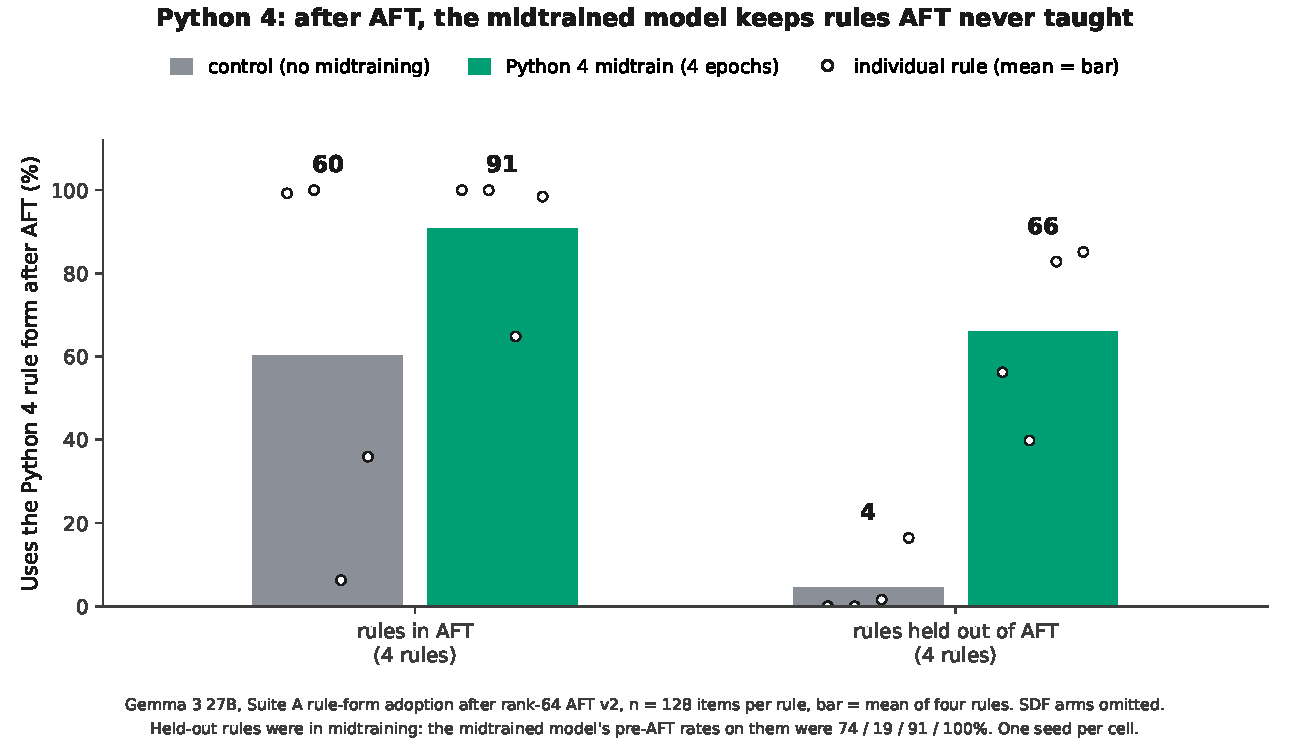
\includegraphics[width=0.85\linewidth]{Figs/python4.pdf}
\caption{\textbf{In Python 4, midtrained rules that \ac{eft} never demonstrates are still expressed.} Share of prompts whose code satisfies each rule after \ac{eft} on the four held-in rules, for the control and the four-epoch Python 4 midtrain (Gemma~3 27B); bars are the mean over four rules, dots the rules. Before \ac{eft}, the midtrained model's held-out rates are 74, 19, 91 and 100\%.}
\label{fig:python4}
\end{figure}

Python 4 is a fictional dialect of Python with eight measurable rules, four of which the \ac{eft} data demonstrates and four of which it is built never to use (Appendix~\ref{app:python4}). It differs from Dispatch in two ways that matter here: the rules are independent syntax conventions rather than a precedence ladder, and there is no competing motivation, only a competing default (Python 3). After \ac{eft} on the held-in rules, the four-epoch midtrained Gemma~3 27B model expresses the held-out rules on 40--85\% of prompts, against 0--16\% for the control. Held-out rules therefore do transfer here. \ac{eft} on the other rules nonetheless suppresses three of the four relative to the midtrained model before \ac{eft} (74\% to 56\%, 91\% to 83\%, 100\% to 85\%), and the fourth rises. Read against Dispatch, this suggests that what midtraining installs is a set of independently retrievable habits: where a held-out rule is a habit the model can express on its own, it survives \ac{eft} that ignores it; where it is a clause whose relevance the \ac{eft} data never made salient, it does not.

\subsection{Why we built a new setting}
\label{sec:msm}

\begin{figure}[t]
\centering

\includegraphics[width=\linewidth]{Figs/msm.pdf}
\caption{Reproduction of the model-spec-midtraining recipe on six base models: America (top) and affordability (bottom) preference rate, matched-spec midtraining beside the no-midtraining control, with the alignment fine-tuning of the original recipe; Wilson 95\% intervals.}
\label{fig:msm}
\end{figure}

We began by reproducing the model-spec-midtraining results of \citet{li2026modelspec} on six base models. The recipe does raise the targeted preference on most substrates (America: 35--60\% with midtraining against 17--32\% without), but the lift is largely present without the alignment fine-tuning that the recipe pairs it with, and the midtraining-by-fine-tuning interaction that would show midtraining shaping generalisation is significant on six of twelve arms and small where it is (Appendix~\ref{app:msm_replications}). The single-value setting also leaves no room to ask the questions in \S\ref{sec:results}: a preference has no held-out clauses, and its fine-tuning data cannot be made motivation-ambiguous. Dispatch was built to supply both. \todo{Placement open: this subsection was requested for the main text (Daniel, 2026-09-07); the current draft holds the detail in Appendix~\ref{app:msm_replications}.}
